%----------------------------------------------------------------------------
\chapter{Mérési feladatok}\label{sect:LatexTools}
%----------------------------------------------------------------------------
%
%\begin{figure}[!ht]
%	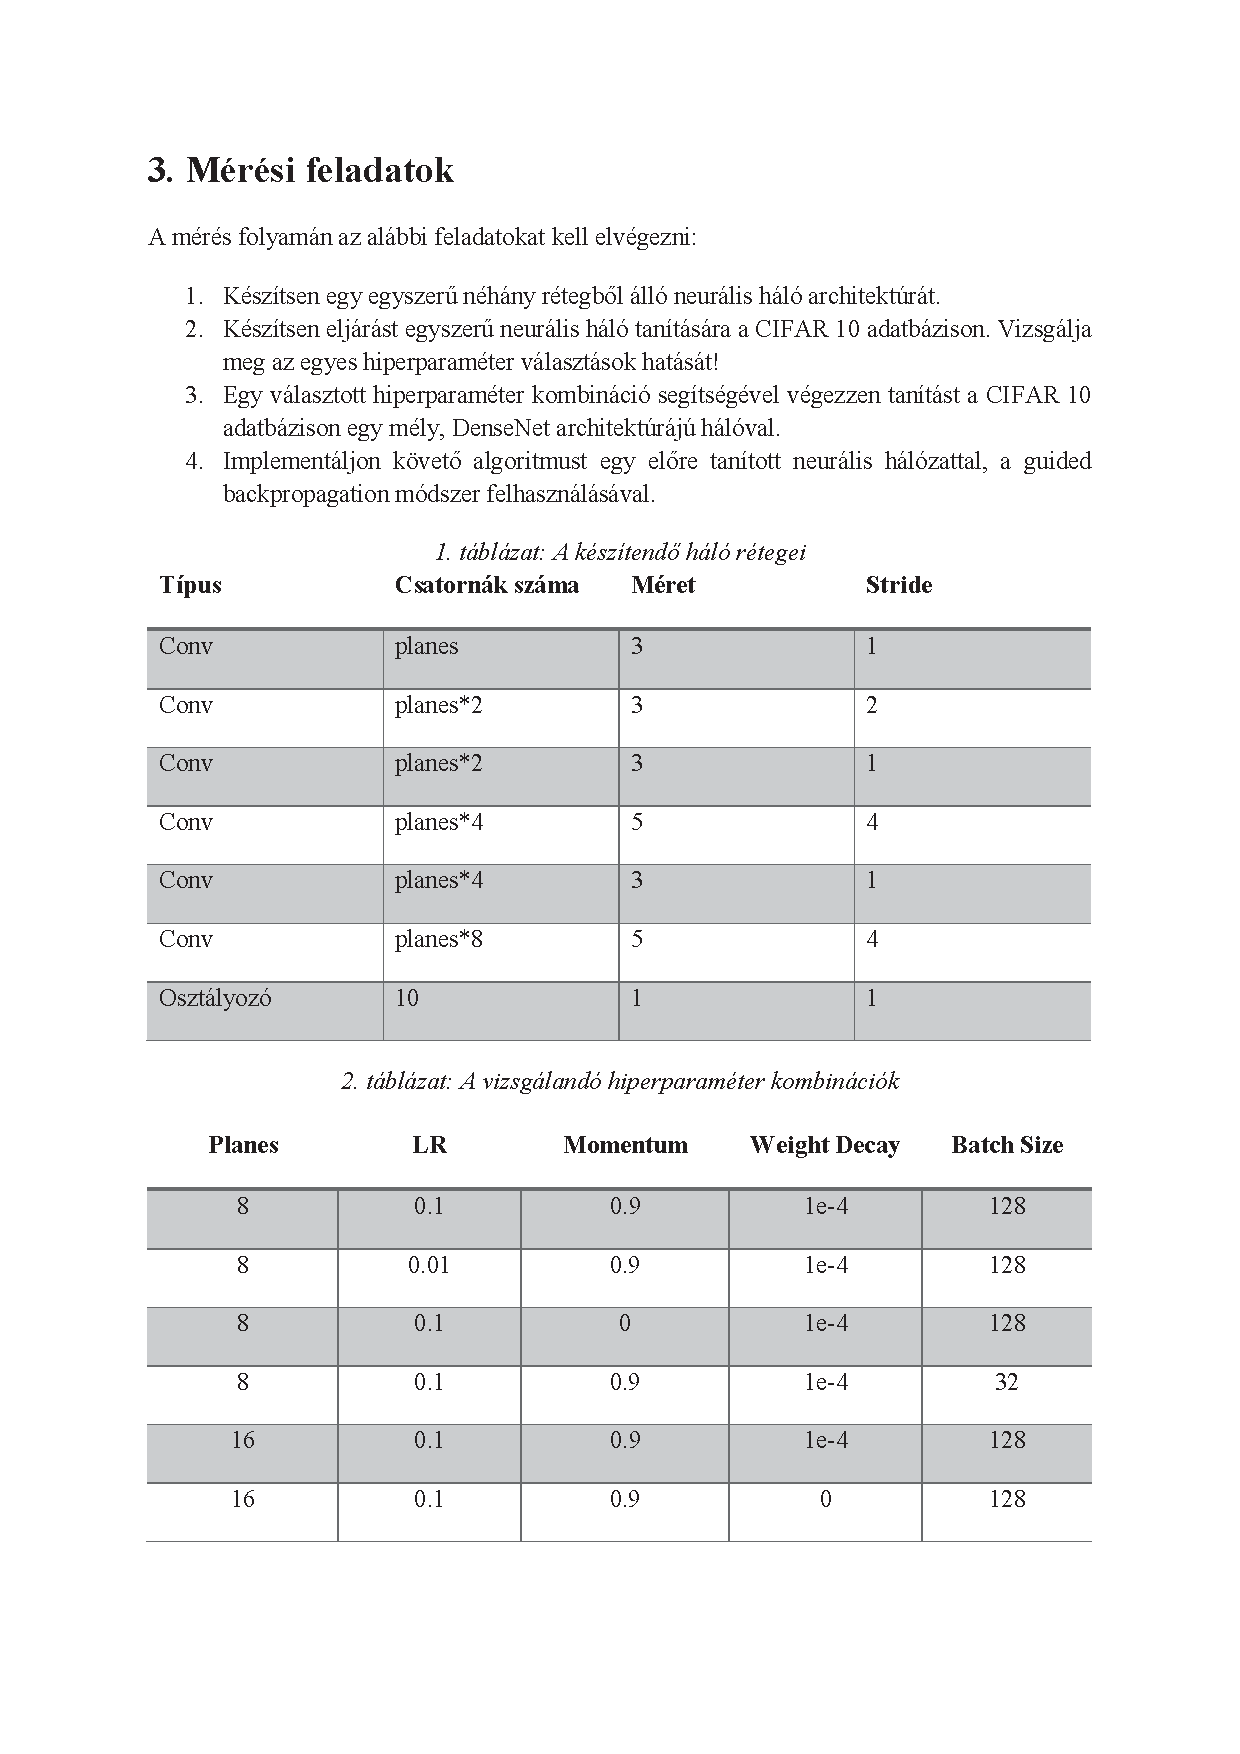
\includegraphics[trim = 25mm 210mm 20mm 33mm,clip, width=150mm,keepaspectratio]{figures/feladatok_m07.pdf}
%	\label{fig:Road-of-a-char}
%\end{figure}

A mérés folyamán az alábbi feladatokat kell elvégezni:
\begin{enumerate}
	\item Swipe gesztusok detektálása:
		\begin{itemize}
			\item A processFrame() függvény arra használható, hogy ellenőrizhessük azt, hogy a Leap Motion detektált-e kezeket. Amennyiben van detektált kéz, a lista továbbítható a processHands() függvény felé.
			\item A processHands() függvény megkapja a kezek listáját, ahol minden kéz esetén tudjuk ellenőrizni, hogy az adott kéz éppen swipe gesztust végez-e. Ehhez ellenőrizzük a kéz mozgásának sebességét (kb 750-1000 határérték megfelelő).
			\item Írjuk a konzolra a swipe gesztusok detektálását.
		\end{itemize}
	\item Döntsük el, hogy egy adott swipe gesztus melyik irányban történik. Ehhez előre definiált jobbra, balra, fel és le vektorokkal tudjuk összehasonlítani a mozgás irányát. Tipp: a Leap::Vector osztály referenciáját érdemes nézegetni. Írjuk ki a swipe irányát is a konzolra.
	\item Detektáljuk, hogy az egyes kezek ökölbe szorított, vagy nyitott állapotban vannak-e.
		\begin{itemize}
			\item Ehhez minden kézre hívjuk meg a grabTest() függvényt, amelyben ezt az ellenőrzést implementáljuk.
			\item Detektáljuk az egyes kezek becsukásának eseményét mind a két kézre külön. Írjuk ki ezeket az eseményeket a konzolra.
		\end{itemize}
	\item Végezzük el a Leap Motion jeleit feldolgozó rendszer és a vezérelni kívánt GUI összekötését.
	\begin{itemize}
		\item A vezérléshez meghívandó üzenetküldő függvények communication.hpp fájlban találhatók.
		\item Az kezek ökölbe szorítására a rendszer a következőképpen reagáljon: amennyiben a bal kezet szorítjuk ökölbe, akkor a rendszer zoomoljon be, ha pedig a jobb kezünket szorítottuk ökölbe, akkor zoomoljon ki.
	\end{itemize}
	
	\item Változtassa meg a rendszer működését az alábbiak szerint:
	\begin{itemize}
		\item Az ökölbe szorítás esetén legyen mindegy, hogy melyik kezet szorítottuk ökölbe, hanem az egy bizonyos időn belül megtörtént kézbecsukások száma adja meg a zoomolás irányát. Egy „klikkre" zoomoljuk be, duplaklikk esetén pedig ki. Tipp: használjon időmérést.
	\end{itemize}
\end{enumerate}
